\Chapter{Szimulációk}

\Section{A szimuláció alakulása paraméterezés függvényében}
A paraméterezést az alkalmazáson belül megjelenő felületről lehet állítani. A következő értékek változtathatóak:
\begin{itemize}
\item{A közlekedési lámpák váltakozásainak ideje, másodpercben megadva}
\item{A szimulációban egyidőben maximálisan résztvevő autóbuszok száma}
\item{A szimulációban egyidőben maximálisan résztvevő személygépjárművek száma}
\item{Két személygépjármű létrehozása közötti eltelt idő, másodpercben mérve}
\item{A város úthálózadának csomópontszáma}
\item{Egy személygépjármű útjának maximális hossza, csomópontokban mérve}
\end{itemize}
Ezen értékek közül a gráf csomópontszámán kívül mindegyik változtatható a város újra generálása nélkül. Az újra generálást egy Generate Anew gombbal lehet elvégezni a felületen.
\begin{figure}[H]
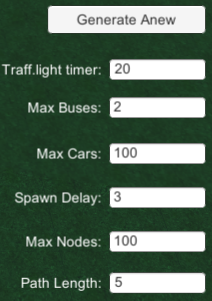
\includegraphics[width=\linewidth]{params.png}
\caption{A paraméterek beállítási felülete, azok alapértelmezett értékeivel}
\label{fig:param}
\end{figure}

Az alapértelmezett paraméterekkel csekély forgalom jön létre egy kis méretű városban. Maga a város képe nagyjából tükrözi egy ilyen méretű város lehetséges elrendezését, az épületek típusai a központ felé bérházak, a peremeknél kertesházak. A szimuláció futása közben a kamerát a W,A,S,D gombokkal lehet mozgatni, valamint az egér görgőjével közelíteni és távolítani.

\subsection{Forgalmi szituációk}
A közlekedési szabályok is megfigyelhetőek az adott objektumoknál, az alábbi képeken ezt szemléltetem.
\begin{figure}[H]
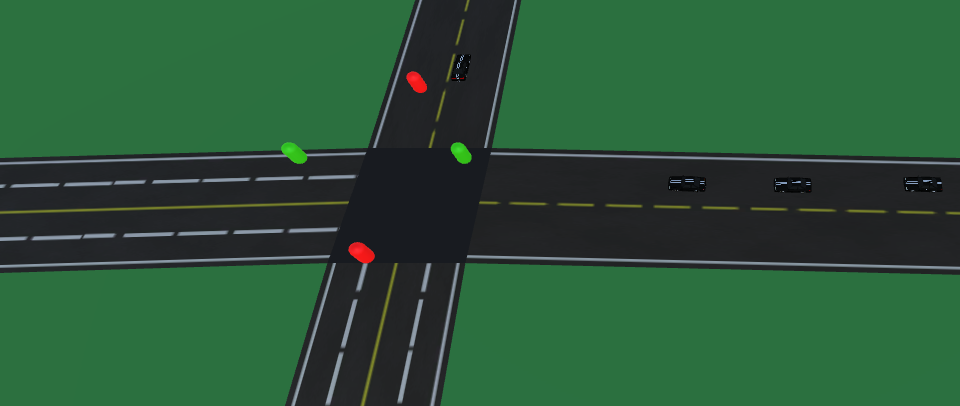
\includegraphics[width=\linewidth]{trafficLight.png}
\caption{Útkereszteződésnél várakozó autók éppen elindulnak}
\label{fig:xroadlight}
\end{figure}
\begin{figure}[H]
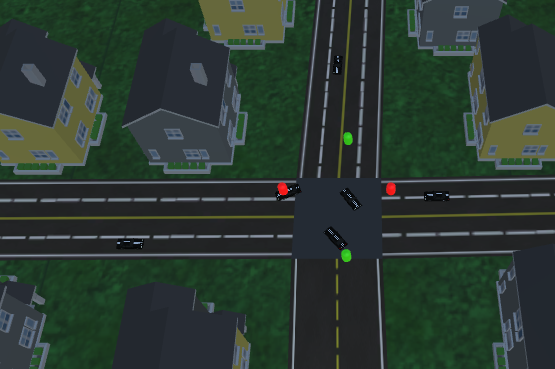
\includegraphics[width=\linewidth]{smalltowntraffic.png}
\caption{Többsávos úton a felülről párhuzamosan érkező autók balra és jobbra kanyarodnak, velük egyidőben szemben jövő autó pedig balra}
\label{fig:multilane}
\end{figure}
\begin{figure}[H]
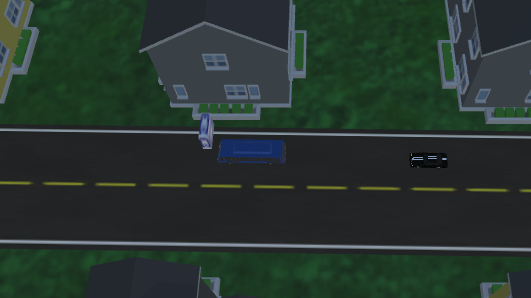
\includegraphics[width=\linewidth]{carwaiting.png}
\caption{Autó az előtte lévő autóbusz elindulását várja}
\label{fig:waiting}
\end{figure}
\begin{figure}[H]
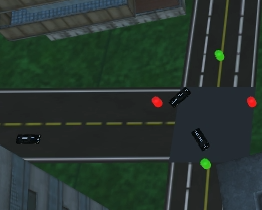
\includegraphics[width=\linewidth]{rofway.png}
\caption{Balra nagy ívben kanyarodó autó elengedi maga előtt a jobbra kis ívben kanyarodót}
\label{fig:rightofway}
\end{figure}

\subsection{Úthálózat mérete}
A generálás méretét tekintve nagyobb városoknál is elvártan működik. A legnagyobb méret amivel teszteltem, az egy 2000 csomópontból álló város. Ezt körülbelül 3 másodperc alatt generálja le egy átlagos számítógépen.
\begin{figure}[H]
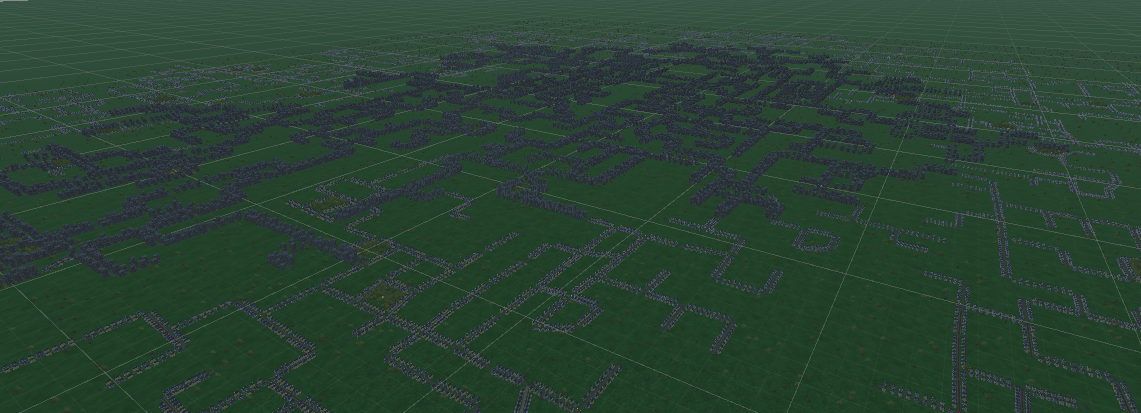
\includegraphics[width=\linewidth]{verybig.png}
\caption{Egy kétezer csomópontból álló város képe}
\label{fig:verybigcity}
\end{figure}

Kipróbáltam valamint egy kisebb, 10 csomópontból álló községet is, megjelenésében és funkcionalitásában ez is megfelelő.
\begin{figure}[H]
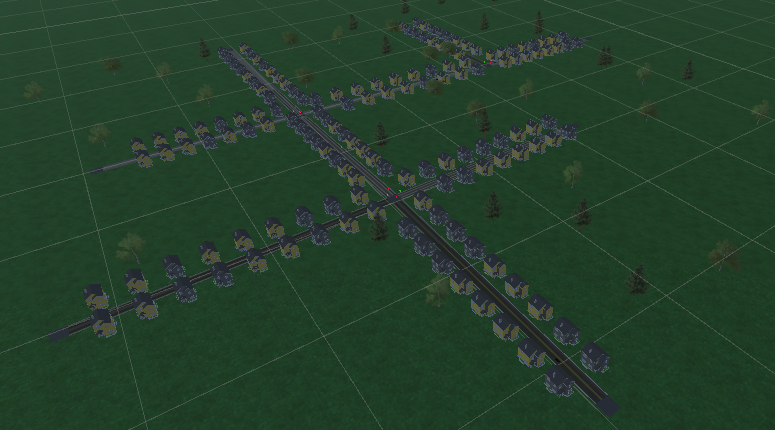
\includegraphics[width=\linewidth]{village.png}
\caption{Tíz csomópontból álló község}
\label{fig:smalltown}
\end{figure}

\subsection{A forgalom sűrűsége az úthálózat méretének függvényében}
A minimális egy másodperces késleltetés miatt az autók létrehozását illetően könnyebbnek találtam a forgalom vizsgálatát egy kisebb, nagyjából 20 csomópontból álló úthálózaton.

Itt észrevehető hogy átlagos forgalom akkor kezd el kialakulni, ha a ötször annyi mennyiségű jármű van az utakon, mint amennyi csomópontból áll az úthálózat. Ez a paraméterezés még nem okoz forgalmi dugót.
A jelzőlámpák váltási idejét felnövelve 40 másodpercre minimális lassulás észlelhető, de ezt ellensúlyozza az, hogy kevesebbszer kell megállnia egy autónak, ha sokáig egyenesen halad.
\begin{figure}[H]
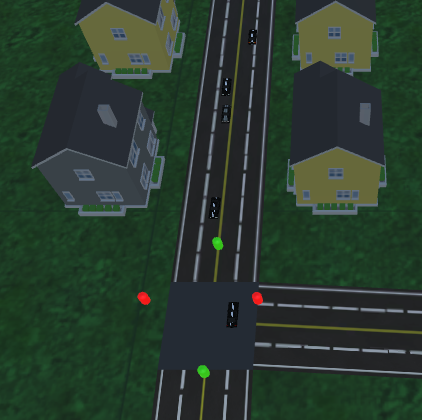
\includegraphics[width=\linewidth]{increasedtraffic.png}
\caption{Nemrég váltott jelzőlámpa előtt várakozik három autó (20 csomópont 100 autóval)}
\label{fig:trafficbigger}
\end{figure}

A parkok is viszonylag rendesen generálódnak, főleg a nagyobb méretű városokban figyelhető ez meg.
\begin{figure}[H]
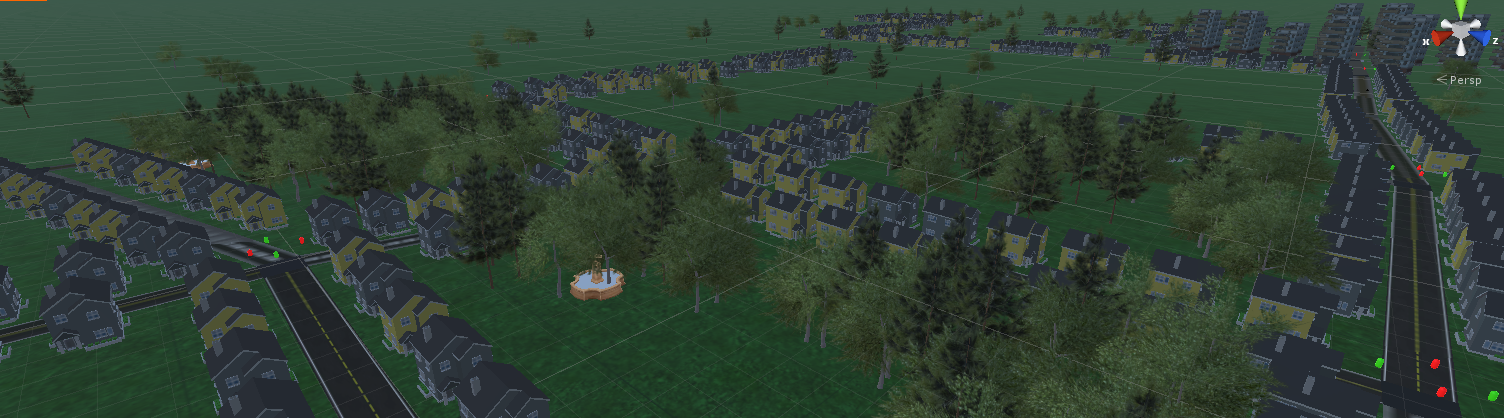
\includegraphics[width=\linewidth]{parks.png}
\caption{Parkok egymás mellett egy város szélén}
\label{fig:parks}
\end{figure}